\section{پروژه دوم (بخش دوم): یادگیری انتقالی (\lr{Transfer Learning}) با \lr{MobileNetV2}}
با توجه به محدودیت داده‌های آموزشی و عملکرد متوسط شبکه‌ی آموزش‌دیده از پایه (دقت $59.41\%$)، در این بخش از تکنیک یادگیری انتقالی استفاده کردیم. هدف، بهره‌گیری از دانشی است که یک مدل بزرگ‌تر روی میلیون‌ها تصویر به دست آورده و انتقال آن به مسئله‌ی دسته‌بندی ۱۷ کلاس گل است.

\vspace{0.4cm}
\subsection{معماری شبکه و پیش‌پردازش}

برای این منظور از مدل \lr{MobileNetV2} استفاده شد که علاوه بر دقت بالا، به دلیل استفاده از \lr{Depthwise Separable Convolutions} بسیار سبک و سریع است و برای محیط‌هایی با منابع محدود ایده‌آل می‌باشد.

\begin{stepbox}
\field{تغییرات معماری و تطبیق ورودی}{
\begin{itemize}
    \item \textbf{لایه پیش‌پردازش:} به‌جای تقسیم ساده‌ی مقادیر پیکسل‌ها بر ۲۵۵، از تابع اختصاصی \lr{\texttt{preprocess\_input}} مربوط به \lr{MobileNetV2} استفاده شد تا ورودی‌ها دقیقاً مطابق با استانداردی باشند که مدل اولیه روی آن آموزش دیده است (محدوده $-1$ تا $1$).
    \item \textbf{حذف سر شبکه (\lr{Include Top = False}):} لایه‌های طبقه‌بند اصلی شبکه‌ی \lr{ImageNet} حذف شدند و به‌جای آن یک لایه‌ی \lr{GlobalAveragePooling2D}، یک لایه‌ی \lr{Dropout} (با نرخ $0.4$) و یک لایه‌ی متراکم ۱۷ نودی با فعال‌ساز \lr{Softmax} اضافه گردید.
\end{itemize}
تعداد کل پارامترهای این شبکه‌ی جدید \textbf{$2,279,761$} است.
}
\end{stepbox}

\vspace{0.4cm}
\subsection{استراتژی آموزش دو فازی (\lr{Two-Phase Training})}

برای جلوگیری از تخریب وزن‌های ازپیش‌آموزش‌دیده (\lr{Catastrophic Forgetting})، فرآیند آموزش در دو فاز مجزا و مهندسی‌شده انجام گرفت:

\begin{itemize}
    \item \textbf{فاز اول (استخراج ویژگی - \lr{Feature Extraction}):} در این فاز، تمامی لایه‌های \lr{MobileNetV2} فریز شدند (\lr{Trainable = False}). تنها لایه‌ی نهایی طبقه بند با بهینه‌ساز \lr{Adam} و نرخ یادگیری نسبتاً بالای $0.001$ به مدت ۲۰ اپوک آموزش دید. 
    \item \textbf{فاز دوم (تنظیم دقیق - \lr{Fine-Tuning}):} پس از همگرایی لایه‌ی نهایی، لایه‌های پایه‌ی \lr{MobileNetV2} از حالت فریز خارج شدند (\lr{Trainable = True}). این بار مدل با نرخ یادگیری بسیار کوچک $10^{-5}$ آموزش دید تا وزن‌های پایه‌ای شبکه به‌آرامی با ویژگی‌های خاصِ گل‌ها سازگار شوند.
\end{itemize}

\begin{figure}[h!]
    \centering
    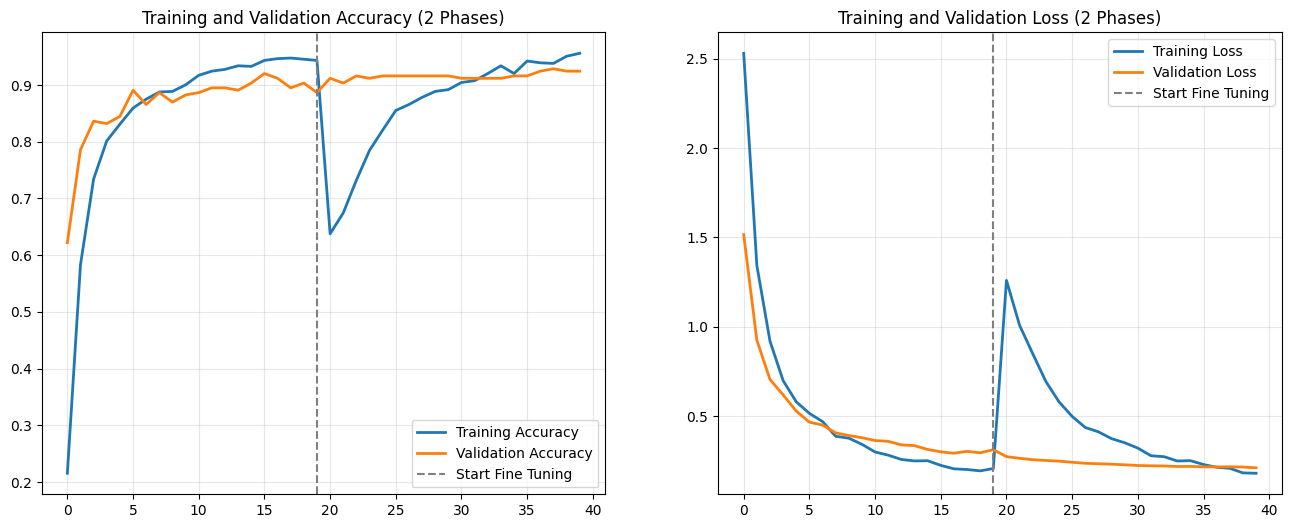
\includegraphics[width=0.95\textwidth]{images/tl_history.png}
    \caption{روند تغییرات دقت (چپ) و تابع زیان (راست) در دو فاز استخراج ویژگی و تنظیم دقیق (خط‌چین خاکستری محل شروع فاز دوم را نشان می‌دهد)}
    \label{fig:tl_history}
\end{figure}

در هر دو فاز از \lr{EarlyStopping} با پارامتر \lr{patience=6} استفاده شد تا همواره بهترین وزن‌ها بازیابی شوند. همان‌طور که در شکل \ref{fig:tl_history} مشخص است، مدل بلافاصله در اپوک‌های ابتدایی به دقت بالایی می‌رسد که نشان‌دهنده‌ی قدرت \lr{Transfer Learning} است.

\vspace{0.4cm}
\subsection{ارزیابی نهایی و جهش عملکرد}

مدل نهایی روی داده‌های آزمون (\lr{Test Set}) ارزیابی شد و به \textbf{دقت فوق‌العاده‌ی $89.41\%$} و \textbf{خطای $0.3791$} دست یافت. این یعنی تقریباً ۳۰ درصد بهبود مطلق نسبت به شبکه‌ی پایه!

\begin{figure}[h!]
    \centering
    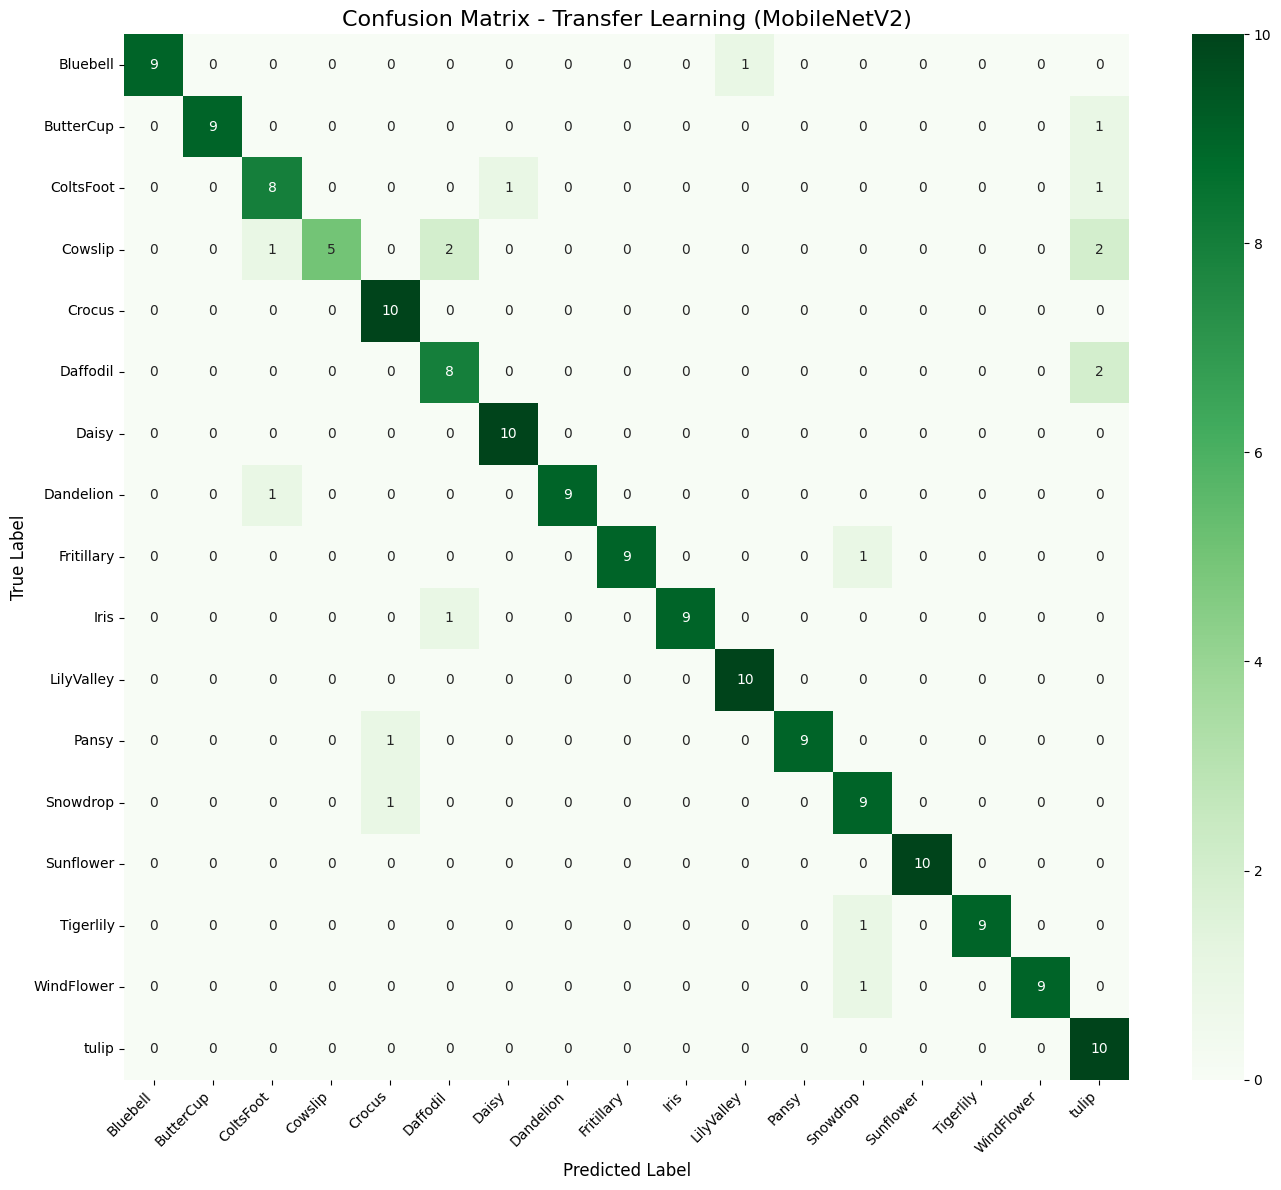
\includegraphics[width=0.85\textwidth]{images/tl_conf_matrix.png}
    \caption{ماتریس درهم‌ریختگی عملکرد مدل \lr{MobileNetV2} روی ۱۷ کلاس تصویر}
    \label{fig:tl_conf_matrix}
\end{figure}

\begin{notebox}[تحلیل گزارش دسته‌بندی]
طبق گزارش استخراج شده، میانگین وزن‌دار \lr{F1-Score} به عدد \textbf{$0.89$} رسیده است. نکته‌ی جالب، عملکرد بی‌نقص مدل روی گل آفتاب‌گردان (\lr{Sunflower}) با \lr{F1-Score} برابر با $1.00$ است که در مدل قبلی یکی از نقاط ضعف اساسی محسوب می‌شد. ضعیف‌ترین عملکرد مربوط به کلاس \lr{Cowslip} (پامچال) با \lr{F1} معادل $0.67$ می‌باشد.
\end{notebox}

\vspace{0.4cm}
\subsection{آزمون در شرایط واقعی (\lr{Inference}) و تحلیل رفتار مدل}

برای مقایسه‌ی عادلانه‌تر، دقیقاً همان ۴ تصویر مرحله‌ی قبل به مدل انتقال یادگیری داده شد:

\vspace{0.3cm}
\begin{figure}[h!]
\centering
\begin{subfigure}{0.24\textwidth}
    \centering
    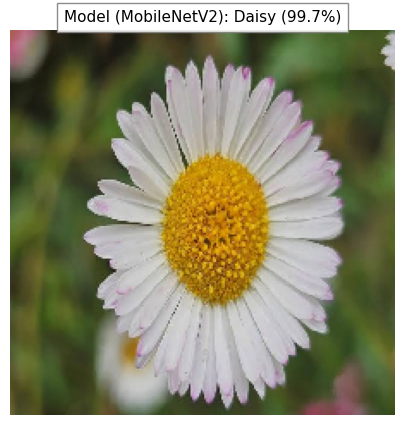
\includegraphics[width=\textwidth]{images/tl_test1.png}
\end{subfigure}
\hfill
\begin{subfigure}{0.24\textwidth}
    \centering
    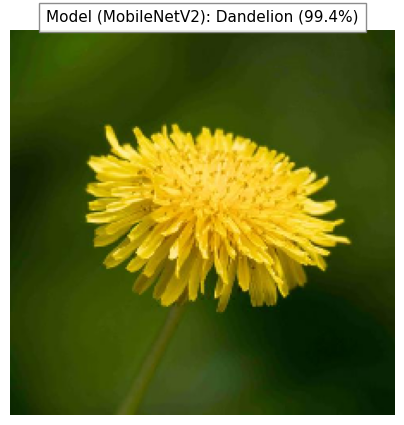
\includegraphics[width=\textwidth]{images/tl_test2.png}
\end{subfigure}
\hfill
\begin{subfigure}{0.24\textwidth}
    \centering
    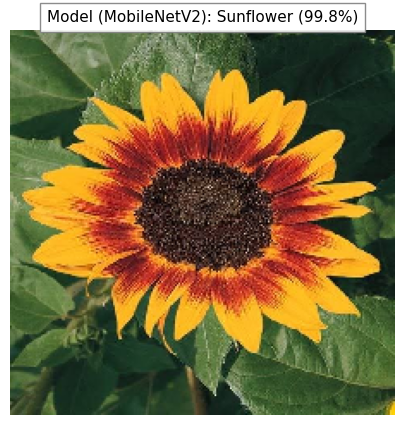
\includegraphics[width=\textwidth]{images/tl_test3.png}
\end{subfigure}
\hfill
\begin{subfigure}{0.24\textwidth}
    \centering
    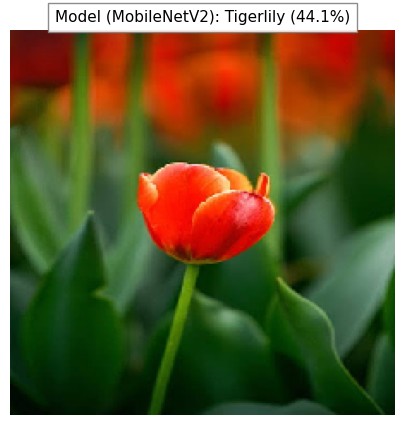
\includegraphics[width=\textwidth]{images/tl_test4.png}
\end{subfigure}
\caption{نتایج پیش‌بینی مدل انتقال یادگیری. (مشکل گل آفتاب‌گردان حل شده و میزان اطمینان مدل در پیش‌بینی اشتباه لاله به شکل منطقی کاهش یافته است)}
\label{fig:tl_inference}
\end{figure}

\begin{tipbox}[کالیبراسیون و عدم قطعیت (\lr{Uncertainty Calibration})]
در مدل شبکه‌ی پیچشیِ پایه‌ی ما (بخش قبل)، تصویر گل لاله به‌اشتباه با اطمینان نزدیک به $100\%$ به‌عنوان \lr{Tigerlily} تشخیص داده شد (یک اشتباه با اعتمادبه‌نفس بالا!). اما در مدل \lr{MobileNetV2}، با وجود اینکه مدل هنوز نتوانسته این لاله را به‌درستی دسته‌بندی کند، اما میزان اطمینان آن به \textbf{$44.1\%$} افت کرده است. 
این اتفاق در محیط‌های عملیاتی بسیار ارزشمند است؛ زیرا نشان می‌دهد مدل ما \lr{Calibrated} شده و در مواقعی که تصویر مبهم است، "می‌داند که نمی‌داند" و با یک توزیع احتمال پخش‌شده (\lr{Smoothed Probability})، از ارائه‌ی پاسخ‌های قطعیِ اشتباه پرهیز می‌کند.
\end{tipbox}